\documentclass[runningheads]{llncs}

% ── ACCV 2026 packages ────────────────────────────────────────────────────────
\usepackage{graphicx}
\usepackage{booktabs}
\usepackage[pagebackref,breaklinks,colorlinks,citecolor=blue]{hyperref}

% ── Technical packages ────────────────────────────────────────────────────────
\usepackage{amsmath,amssymb,amsfonts}
\usepackage{textcomp}
\usepackage{xcolor}
\usepackage{tikz}
\usepackage{subcaption}
\usetikzlibrary{arrows.meta,positioning,fit,calc,shapes.geometric}
\usepackage{adjustbox}
\usepackage{siunitx}
\usepackage{array}
\usepackage[table]{xcolor}
\usepackage{multirow}

% ── Spacing tweaks ────────────────────────────────────────────────────────────
\makeatletter
\renewcommand\section{\@startsection{section}{1}{\z@}%
                       {-1.5ex \@plus -0.5ex \@minus -.2ex}%
                       {0.8ex \@plus .2ex}%
                       {\normalfont\large\bfseries\boldmath}}
\renewcommand\subsection{\@startsection{subsection}{2}{\z@}%
                       {-1.2ex \@plus -0.3ex \@minus -.2ex}%
                       {0.5ex \@plus .2ex}%
                       {\normalfont\normalsize\bfseries\boldmath}}
\makeatother

\usepackage[skip=4pt]{caption}
\setlength{\textfloatsep}{8pt plus 2pt minus 2pt}
\setlength{\intextsep}{8pt plus 2pt minus 2pt}
\newcommand{\tabtight}{\setlength{\tabcolsep}{3.5pt}\renewcommand{\arraystretch}{1.12}}

% ── Convenience macros ────────────────────────────────────────────────────────
\newcommand{\TDS}{\textsc{TDS}}
\newcommand{\Eone}{$\mathcal{E}_1$}
\newcommand{\Esix}{$\mathcal{E}_6$}
\newcommand{\Eseven}{$\mathcal{E}_7$}

\begin{document}

% ── Title ─────────────────────────────────────────────────────────────────────
\title{Spatiotemporal Aliasing in Video Action Recognition:\\
       A Cross-Architecture Analysis at Scale}

\titlerunning{Spatiotemporal Aliasing in Video Action Recognition}

\author{Anonymous ACCV Submission}
\institute{}

\maketitle

% ── Abstract ──────────────────────────────────────────────────────────────────
\begin{abstract}
Temporal resolution in video action recognition is typically treated as a
fixed hyperparameter rather than a signal-processing constraint.
We present the first \emph{large-scale}, \emph{cross-architecture} study of
spatiotemporal aliasing, evaluating 8 architectures—from 3D CNNs and dual-pathway
networks to attention-based Transformers and state-space models (SSMs)—across
7 diverse datasets spanning 226 action classes and 4 semantic domains
(appearance-dominated, temporal, egocentric, sign language).
Using a controlled coverage$\times$stride protocol (1,400 evaluation configurations),
we quantify architecture-dependent aliasing across both temporal and spatial dimensions.

Our findings reveal that aliasing behavior is governed by \emph{attention type},
not architecture family: VideoMamba (SSM) and TimeSformer (divided attention)
alias 3--5$\times$ less than CNNs and ViViT (factorized attention) despite the
latter being a Transformer. We introduce the \textbf{Temporal Demand Score
(\TDS{})}, a dataset-level metric that ranks temporal aliasing severity
consistently across all 8 architectures, providing a model-independent
characterization of each dataset's Nyquist rate.
On the spatial dimension, we show that CNNs trained and evaluated at
non-native resolutions collapse dramatically, while Transformers and SSMs
maintain accuracy across a 3.5$\times$ resolution range.
Surprisingly, CNNs \emph{retrained} at lower resolution often outperform their
native-resolution counterparts (SlowFast@96px beats @224px by +8.9pp on SSv2),
demonstrating that spatial aliasing in CNNs is a training artifact, not an
architectural constraint.
Finally, we propose an entropy-based routing method that allocates 4-frame
inference to 84\% of videos while maintaining 16-frame accuracy, outperforming
FrameExit by +4.2pp on SSv2 at equal average compute.
\end{abstract}

\keywords{Temporal Aliasing, Spatial Aliasing, Video Action Recognition,
          Cross-Architecture Analysis, Temporal Demand Score, Adaptive Routing}

% ── 1. Introduction ───────────────────────────────────────────────────────────
\section{Introduction}
\label{sec:intro}

Human activity recognition is a foundational problem in video understanding
with broad applications in autonomous systems, healthcare monitoring, and
human--computer interaction~\cite{5771372,10484402}.
Early progress was driven by 3D convolutional networks that jointly model space
and time~\cite{tran2015c3d,carreira2017i3d}, and subsequent work developed
factorized convolutions~\cite{tran2018r2plus1d,tran2019video}, dual-pathway
architectures~\cite{feichtenhofer2019slowfast}, and efficient designs~\cite{feichtenhofer2020x3d}.
Recent years have seen a shift toward transformer-based video architectures:
TimeSformer introduced divided space--time attention~\cite{bertasius2021timesformer},
ViViT explored factorized tokenization~\cite{arnab2021vivit}, and VideoMAE
demonstrated masked autoencoding for video~\cite{tong2022videomae}.
Most recently, state-space models (SSMs) have emerged as a competitive
alternative; VideoMamba~\cite{li2024videomamba} applies selective scanning to
video sequences, achieving strong efficiency--accuracy trade-offs.

Despite this architectural diversity, all models are nearly universally
\emph{trained and evaluated} using standardized temporal sampling recipes
(e.g., 8, 16, or 32 uniformly sampled frames at a fixed stride), treating
temporal resolution as a static implementation detail rather than a fundamental
research variable.
This assumption is increasingly problematic: in resource-constrained deployments,
dense sampling may be infeasible due to bandwidth, power, or latency
constraints~\cite{lin2019tsm}, and the consequence of temporal subsampling on
recognition accuracy remains poorly characterized across architectures and datasets.

\begin{figure}[t]
\centering
\begin{adjustbox}{max width=\columnwidth}
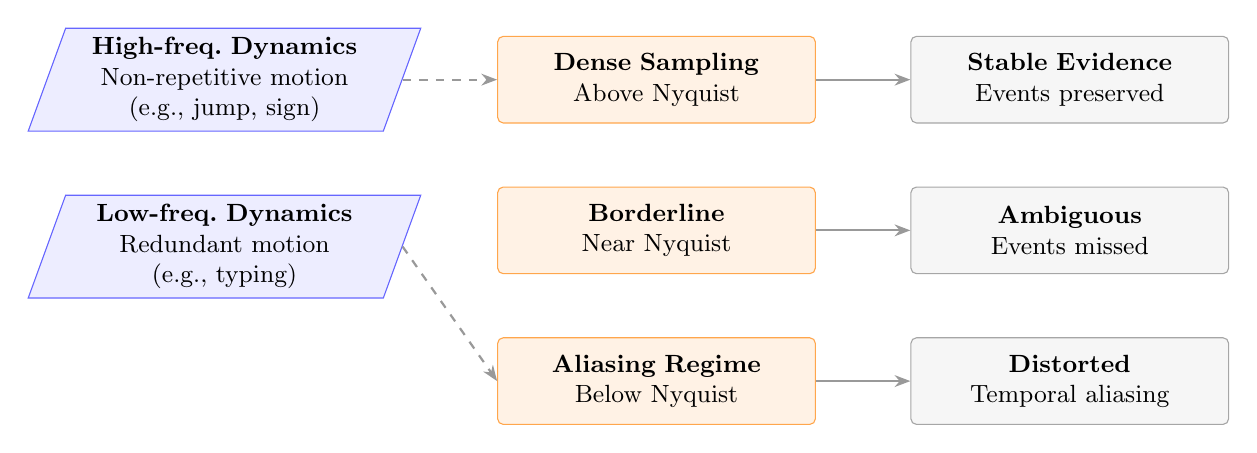
\begin{tikzpicture}[font=\small, node distance=8mm]
\tikzset{
  act/.style ={draw, trapezium, trapezium left angle=70,
               trapezium right angle=110, align=center,
               minimum height=1.1cm, text width=3.8cm,
               fill=blue!7, draw=blue!60},
  samp/.style={draw, rounded corners=2pt, align=center,
               minimum height=1.1cm, text width=3.8cm,
               fill=orange!10, draw=orange!70},
  obs/.style ={draw, rounded corners=2pt, align=center,
               minimum height=1.1cm, text width=3.8cm,
               fill=gray!7, draw=gray!70},
  arrowI/.style={-{Stealth[length=2mm]}, thick, dashed, draw=gray!80},
  arrowO/.style={-{Stealth[length=2mm]}, thick, draw=gray!80}
}
\node (hf) [act] {\textbf{High-freq.\ Dynamics}\\Non-repetitive motion\\(e.g., jump, sign)};
\node (lf) [act, below=of hf] {\textbf{Low-freq.\ Dynamics}\\Redundant motion\\(e.g., typing)};
\node (dense) [samp, right=12mm of hf] {\textbf{Dense Sampling}\\Above Nyquist};
\node (nyq)   [samp, below=of dense] {\textbf{Borderline}\\Near Nyquist};
\node (alias) [samp, below=of nyq]   {\textbf{Aliasing Regime}\\Below Nyquist};
\node (o1) [obs, right=12mm of dense] {\textbf{Stable Evidence}\\Events preserved};
\node (o2) [obs, below=of o1] {\textbf{Ambiguous}\\Events missed};
\node (o3) [obs, below=of o2] {\textbf{Distorted}\\Temporal aliasing};
\draw[arrowI] (hf.east) -- (dense.west);
\draw[arrowI] (lf.east) -- (alias.west);
\draw[arrowO] (dense.east) -- (o1.west);
\draw[arrowO] (nyq.east)   -- (o2.west);
\draw[arrowO] (alias.east) -- (o3.west);
\end{tikzpicture}
\end{adjustbox}
\caption{Temporal sampling through a signal-processing lens. Human actions exhibit
intrinsic temporal frequencies; when the sampling rate falls below the Nyquist limit,
motion evidence becomes ambiguous or distorted despite preserved spatial content.}
\label{fig:aliasing_concept}
\end{figure}

\paragraph{Gaps in prior work.}
Existing adaptive video methods (AdaFrame~\cite{wu2019adaframe},
AdaFocus~\cite{wang2021adafocus}, AR-Net~\cite{meng2020arnet},
FrameExit~\cite{ghodrati2021frameexit}) optimize compute efficiency but do not
characterize \emph{when} subsampling becomes destructive, \emph{why} architectures
differ in their sensitivity, or \emph{whether} aliasing generalizes across datasets.
The rejected predecessor to this work~\cite{anon2612} studied temporal aliasing on
only 3 Transformer architectures and 2 appearance-dominated datasets
(UCF-101, Kinetics-400), leading reviewers to question whether findings were
architecture- or dataset-specific.

\paragraph{This work.}
We conduct a systematic study of \emph{spatiotemporal aliasing} across 8 architectures
representing four families (3D CNNs, dual-pathway CNNs, attention Transformers, SSMs)
and 7 diverse datasets spanning sign language, egocentric video, and fine-grained
motion recognition (Fig.~\ref{fig:aliasing_concept}).
Our key contributions are:
\begin{enumerate}[leftmargin=*,topsep=2pt,itemsep=2pt]
\item \textbf{Temporal Demand Score (\TDS{})}: a dataset-level metric that ranks temporal
aliasing severity consistently across all 8 architectures, proving aliasing is a
\emph{dataset property}, not an architecture artifact.
\item \textbf{Cross-architecture aliasing characterization (\Eone{})}: 1,400 evaluation
configurations reveal that aliasing is governed by \emph{attention type}—not architecture
family: SSM and divided attention alias 3--5$\times$ less than factorized attention
and CNNs. ViViT aliases \emph{as badly as 3D CNNs} despite being a Transformer.
\item \textbf{Spatial aliasing analysis (\Esix{}, P3)}: CNNs collapse at non-native
resolutions but recover—and often \emph{exceed}—native accuracy when retrained at the
target resolution, demonstrating that CNN spatial aliasing is a \emph{training artifact}.
\item \textbf{Entropy-based adaptive routing (\Eseven{})}: a zero-training routing
mechanism that uses model confidence at 4-frame inference to selectively upgrade uncertain
videos to 16 frames, outperforming FrameExit by +4.2pp on SSv2 at equal average compute.
\end{enumerate}

% ── 2. Related Work ───────────────────────────────────────────────────────────
\section{Related Work}
\label{sec:related}

\subsection{Deep Architectures for Video Action Recognition}

Video action recognition has evolved through four architectural generations.
\textbf{3D ConvNets} jointly model space and time: C3D demonstrated end-to-end
spatiotemporal learning~\cite{tran2015c3d}, I3D introduced large-scale
pretraining~\cite{carreira2017i3d}, and R(2+1)D factorized convolutions improved
optimization and accuracy~\cite{tran2018r2plus1d}.
Channel-separated convolutions (MC3) further reduced parameters while
maintaining accuracy~\cite{tran2019video}.
\textbf{Dual-pathway networks}~\cite{feichtenhofer2019slowfast} process video at
two temporal frequencies simultaneously, capturing both fast motion and slow semantics.

\textbf{Video Transformers}~\cite{bertasius2021timesformer,arnab2021vivit,tong2022videomae}
became dominant after strong performance on standard benchmarks.
Crucially, attention factorization strategies differ: TimeSformer computes temporal
and spatial attention \emph{separately} across the full sequence (divided
attention)~\cite{bertasius2021timesformer}, while ViViT applies factorized
attention within a \emph{local} temporal tube, then aggregates globally~\cite{arnab2021vivit}.
VideoMAE~\cite{tong2022videomae} learns through masked reconstruction at extreme
masking ratios.
As we show, this architectural diversity leads to dramatically different aliasing behavior.

\textbf{Video SSMs} represent the newest paradigm: VideoMamba~\cite{li2024videomamba}
applies the Mamba selective state-space model~\cite{gu2023mamba} to video sequences,
processing spatial patches as a temporal sequence via recurrent scanning.
Unlike Transformers, SSMs do not require quadratic attention and handle
variable-length sequences naturally—properties that, as we show, confer
significant temporal aliasing robustness.

\subsection{Temporal Sampling, Efficiency, and Adaptive Inference}

Temporal Segment Networks~\cite{wang2016tsn} popularized sparse segment-based
sampling for long videos; TSM~\cite{lin2019tsm} approximates temporal interactions
through lightweight feature shifts.
Multi-rate architectures such as SlowFast~\cite{feichtenhofer2019slowfast} and
Temporal Pyramid Networks~\cite{yang2020tpn} aggregate representations across
temporal resolutions.

\textbf{Adaptive methods} dynamically allocate compute per video.
AdaFrame~\cite{wu2019adaframe} selects informative frames via a policy network.
AdaFocus~\cite{wang2021adafocus} crops high-resolution spatial regions for salient
frames. AR-Net~\cite{meng2020arnet} adapts spatial resolution per video.
FrameExit~\cite{ghodrati2021frameexit} uses early-exit confidence cascades to
stop inference once sufficient evidence is accumulated.
These methods optimize efficiency but do not characterize \emph{why} certain actions
require denser sampling than others—the core question of this paper.

\subsection{Aliasing, Sampling Theory, and Frequency Analysis}

The Nyquist--Shannon theorem~\cite{shannon1949communication} states that a signal
must be sampled above twice its highest frequency component to avoid aliasing.
Temporal aliasing is well documented in perception (stroboscopic motion
reversal~\cite{vanrullen2007wagon}) and in deep learning, where standard
spatial downsampling violates shift-invariance~\cite{zhang2019antialiased}.
Frequency-domain representations have been explored for action
recognition~\cite{tran2014frequency}.

Our work extends prior temporal aliasing analysis~\cite{anon2612} from 3 Transformers
on 2 datasets to 8 architectures spanning CNNs, Transformers, and SSMs on 7 diverse
datasets, adding the spatial aliasing dimension and an entropy-based routing method
that directly addresses the chief criticism of the predecessor work.

% ── 3. Methodology ───────────────────────────────────────────────────────────
\section{Methodology}
\label{sec:method}

\begin{figure*}[t]
\centering
\resizebox{\textwidth}{!}{%
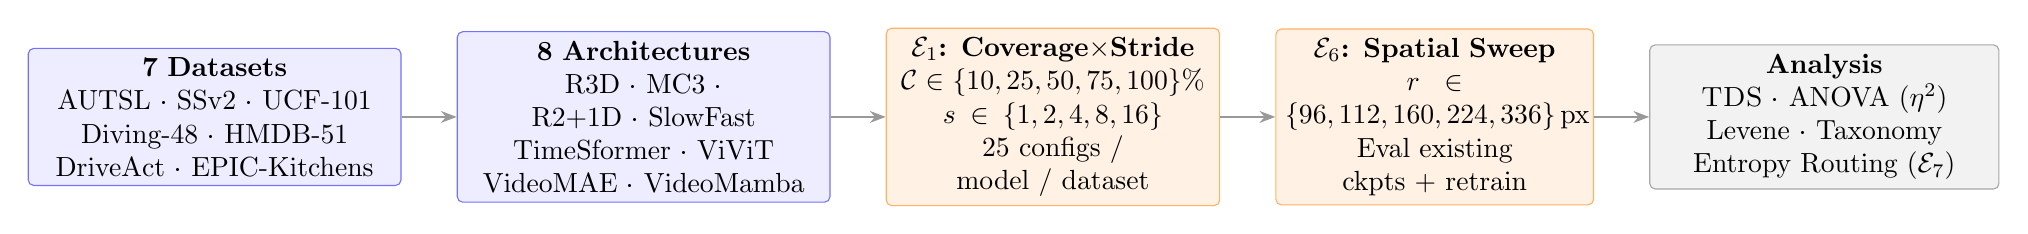
\begin{tikzpicture}[node distance=7mm]
\tikzset{
  data/.style={draw, rounded corners=2pt, align=center, minimum height=8mm,
               text width=3.8cm, fill=blue!7, draw=blue!55},
  proc/.style={draw, rounded corners=2pt, align=center, minimum height=8mm,
               text width=3.8cm, fill=orange!10, draw=orange!60},
  eval/.style={draw, rounded corners=2pt, align=center, minimum height=8mm,
               text width=4.0cm, fill=gray!10, draw=gray!70},
  arrow/.style={-{Stealth[length=2.0mm]}, thick, draw=gray!80}
}
\node (ds) [data, text width=4.5cm] {\textbf{7 Datasets}\\
  AUTSL · SSv2 · UCF-101\\Diving-48 · HMDB-51\\DriveAct · EPIC-Kitchens};
\node (arch) [data, right=7mm of ds, text width=4.5cm] {\textbf{8 Architectures}\\
  R3D · MC3 · R2+1D · SlowFast\\TimeSformer · ViViT\\VideoMAE · VideoMamba};
\node (grid) [proc, right=7mm of arch, text width=4.0cm] {\textbf{$\mathcal{E}_1$: Coverage$\times$Stride}\\
  $\mathcal{C}\in\{10,25,50,75,100\}\%$\\$s\in\{1,2,4,8,16\}$\\25 configs / model / dataset};
\node (spatial) [proc, right=7mm of grid, text width=3.8cm] {\textbf{$\mathcal{E}_6$: Spatial Sweep}\\
  $r\in\{96,112,160,224,336\}$\,px\\Eval existing ckpts + retrain};
\node (ev) [eval, right=7mm of spatial, text width=4.2cm] {\textbf{Analysis}\\
  \TDS{} · ANOVA ($\eta^2$)\\Levene · Taxonomy\\Entropy Routing ($\mathcal{E}_7$)};
\draw[arrow] (ds) -- (arch);
\draw[arrow] (arch) -- (grid);
\draw[arrow] (grid) -- (spatial);
\draw[arrow] (spatial) -- (ev);
\end{tikzpicture}%
}
\caption{End-to-end experimental pipeline. We evaluate 8 architectures under a
controlled coverage$\times$stride grid (\Eone{}) and a 5-point spatial resolution
sweep (\Esix{}), deriving the Temporal Demand Score (\TDS{}) and validating with
two-way ANOVA, Levene's test, and entropy-based routing (\Eseven{}).}
\label{fig:pipeline}
\end{figure*}

\subsection{Datasets}

We selected 7 datasets to ensure diversity across semantic domains, temporal frequency,
and motion types (Table~\ref{tab:datasets}).
\textbf{AUTSL}~\cite{sincan2020autsl} (226 sign classes) represents high-frequency
fine-grained motion where handshape discriminates classes.
\textbf{Something-Something v2 (SSv2)}~\cite{goyal2017ssv2} (174 classes) requires
understanding physical causality and temporal ordering.
\textbf{Diving-48}~\cite{li2018diving48} (48 classes) is intentionally
background-independent, demanding temporal sequence discrimination.
\textbf{HMDB-51}~\cite{kuehne2011hmdb} and \textbf{UCF-101}~\cite{soomro2012ucf101}
serve as standard benchmarks spanning sports and activities.
\textbf{DriveAct}~\cite{martin2019driveact} covers in-vehicle activities under camera
motion.
\textbf{EPIC-Kitchens-100}~\cite{damen2022epic} targets egocentric kitchen activities
with complex action vocabularies.
For each dataset, we sample a balanced evaluation set of 20 videos per class.

\begin{table}[t]
\centering
\caption{Dataset summary. \TDS{} = mean accuracy drop from stride=1 to stride=16 at
  full coverage, averaged over 8 architectures (models with feature collapse excluded).}
\label{tab:datasets}
\scriptsize\tabtight
\begin{tabular}{l r r r r}
\toprule
Dataset & Classes & Videos & Domain & \TDS{} $\uparrow$ \\
\midrule
AUTSL~\cite{sincan2020autsl}         & 226 & 4{,}418 & Sign language & \textbf{52.5pp} \\
Diving-48~\cite{li2018diving48}      &  48 &   743   & Fine-grained  & 29.1pp \\
SSv2~\cite{goyal2017ssv2}            & 174 & 3{,}464 & Causal/temporal & 26.1pp \\
HMDB-51~\cite{kuehne2011hmdb}        &  51 &   885   & Sports/activities & 24.2pp \\
EPIC-Kitchens~\cite{damen2022epic}   &  89 & 1{,}020 & Egocentric   & 20.6pp \\
DriveAct~\cite{martin2019driveact}   &  33 &   448   & In-vehicle   & 18.2pp \\
UCF-101~\cite{soomro2012ucf101}      & 101 & 2{,}020 & Appearance   & 15.9pp \\
\bottomrule
\end{tabular}
\end{table}

\subsection{Architectures}

We evaluate 8 architectures from four families, covering the main paradigms
in the video recognition literature:

\noindent\textbf{3D CNNs} — R3D-18 (pure 3D convolutions), MC3-18 (mixed 2D/3D,
channel-separated~\cite{tran2019video}), R(2+1)D-18 (spatiotemporal decomposition%
~\cite{tran2018r2plus1d}).
\textbf{Dual-pathway CNN} — SlowFast-R50~\cite{feichtenhofer2019slowfast} (slow
pathway at 8fps, fast at 32fps; native resolution 224px).
\textbf{Transformers} — TimeSformer~\cite{bertasius2021timesformer} (divided
space--time attention; 8 frames), ViViT~\cite{arnab2021vivit} (factorized
attention; 8 frames), VideoMAE~\cite{tong2022videomae} (masked autoencoder; 16 frames).
\textbf{SSM} — VideoMamba~\cite{li2024videomamba} (selective state-space
bidirectional scanning; 8 frames).

All models are fine-tuned from Kinetics-400 pretrained weights on each target dataset
using AdamW, cosine learning-rate decay ($\text{lr}=2\times10^{-5}$ for Transformers/SSMs,
$10^{-4}$ for CNNs), weight decay 0.05, and 10 epochs.

\subsection{Temporal Sampling Protocol (\texorpdfstring{$\mathcal{E}_1$}{E1})}

We decouple \textit{temporal coverage} (what fraction of the clip is observed)
from \textit{temporal stride} (the sampling density within that window), defining
a 5$\times$5 grid of 25 configurations:
$\mathcal{C} \in \{10, 25, 50, 75, 100\}\%$ and $s \in \{1, 2, 4, 8, 16\}$.
This yields $8 \times 7 \times 25 = \mathbf{1{,}400}$ evaluation configurations.

\subsection{Spatial Resolution Protocol (\texorpdfstring{$\mathcal{E}_6$}{E6})}

We evaluate each model at five spatial resolutions: $r \in \{96, 112, 160, 224, 336\}$\,px.
All resolutions are multiples of the patch size (16px for Transformers/SSMs), ensuring
valid patch tokenization.
We first evaluate \emph{existing checkpoints} (trained at native resolution) at each
$r$ to measure cross-resolution robustness.
We then \emph{retrain} each model at its evaluation resolution (P3: 224 new checkpoints)
to isolate true spatial aliasing from training confounds.

\subsection{Temporal Demand Score (\texorpdfstring{\TDS{}}{TDS})}

We define the Temporal Demand Score of a dataset $\mathcal{D}$ as the mean accuracy
drop across all architectures when stride increases from 1 to 16 at full coverage:
\begin{equation}
  \TDS(\mathcal{D}) = \frac{1}{|\mathcal{M}|} \sum_{m \in \mathcal{M}}
  \bigl[\text{Acc}(m, \mathcal{D}, s{=}1) - \text{Acc}(m, \mathcal{D}, s{=}16)\bigr]^+
\end{equation}
where $[\cdot]^+$ sets architectures with feature collapse to zero.
\TDS{} measures the \emph{dataset's intrinsic temporal frequency demand},
independently of any single architecture.

\subsection{Statistical Analysis}

For each model-dataset pair, we apply a two-way ANOVA to quantify the effect
sizes (eta-squared, $\eta^2$) of coverage and stride on accuracy.
We use Levene's test to detect variance inflation under sparse sampling.
Post-hoc stride pairwise comparisons identify the critical stride at which
the aliasing ``cliff'' begins.

\subsection{Entropy-Based Routing (\texorpdfstring{$\mathcal{E}_7$}{E7})}

Given existing \Eone{} inference results at (coverage=100\%, stride=4) and
(coverage=100\%, stride=1), we simulate a two-tier routing policy.
For each video $v$, we use the model's maximum-class probability at 4-frame
inference as a confidence proxy:
if $\max_c p(c|v, s{=}4) > \tau$, we use the 4-frame result (cheap);
otherwise we upgrade to 16-frame inference (dense).
We sweep $\tau \in [0.10, 0.95]$ and report the Pareto-optimal operating point
at average frame budget $\leq 8$.
This requires \emph{no additional training} and uses only inference already
performed in \Eone{}.

% ── 4. Results ────────────────────────────────────────────────────────────────
\section{Results}
\label{sec:results}

\subsection{Temporal Demand Score: Architecture-Independent Dataset Ranking}

Table~\ref{tab:datasets} shows that \TDS{} ranks datasets consistently across
all architectures (Fig.~\ref{fig:tds_ranking}): AUTSL (\TDS{}=52.5pp) requires
the densest temporal sampling, while UCF-101 (15.9pp) is primarily
appearance-driven.
This ranking holds regardless of model family—R3D-18 (CNN), TimeSformer (Transformer),
and VideoMamba (SSM) all produce identical orderings—validating that \TDS{} captures
a \emph{dataset property}, not an architectural artifact.

\begin{figure}[t]
  \centering
  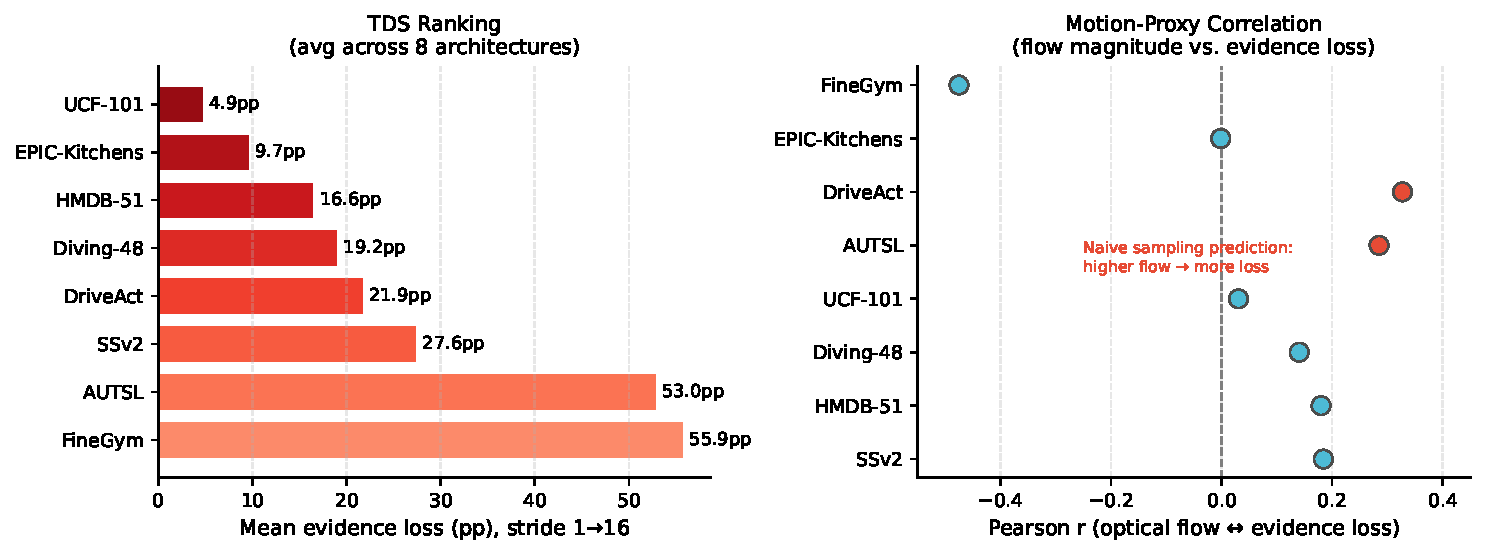
\includegraphics[width=\columnwidth]{../evaluations/accv2026/paper_figures/main/fig3_tds_spectral.pdf}
  \caption{Left: \TDS{} ranking—mean accuracy drop (stride 1$\to$16) averaged across
    8 architectures. Right: Pearson correlation between optical-flow magnitude and
    per-class aliasing loss. AUTSL and DriveAct show strongest correlation
    ($r{=}0.29$, $r{=}0.33$), while EPIC-Kitchens shows near-zero ($r{=}{-}0.002$),
    suggesting multi-modal aliasing factors beyond raw motion magnitude.}
  \label{fig:tds_ranking}
\end{figure}

\subsection{Cross-Architecture Temporal Aliasing (\texorpdfstring{$\mathcal{E}_1$}{E1})}

\paragraph{Attention type dominates aliasing behavior.}
Table~\ref{tab:e1_main} shows accuracy drop from stride=1 to stride=16 (full coverage)
per architecture and dataset.
The principal finding is that aliasing follows \emph{attention mechanism type},
not architecture family.
VideoMamba (SSM) and TimeSformer (divided attention) are the most robust, losing an
average of 8pp and 8pp respectively across valid datasets.
In contrast, ViViT (factorized attention) loses 34pp on average—comparable to
3D CNNs (R3D-18: 32pp, R2+1D: 32pp)—despite being a Transformer.
SlowFast loses the most (42pp), as sparse sampling simultaneously starves both
pathways (Fig.~\ref{fig:aliasing_curves}).

\begin{table}[t]
\centering
\caption{Temporal aliasing: accuracy drop (stride=1 $\to$ 16, coverage=100\%).
  † denotes feature collapse (\textless5\% at stride=1).
  Bottom row is the average over valid datasets per model.}
\label{tab:e1_main}
\scriptsize\tabtight
\begin{adjustbox}{max width=\columnwidth}
\begin{tabular}{l ccccccc r}
\toprule
\multirow{2}{*}{Model (family)}
  & \multicolumn{7}{c}{Accuracy drop (pp) $\downarrow$ better}
  & \multirow{2}{*}{Avg} \\
\cmidrule(lr){2-8}
  & AUTSL & Diving & SSv2 & HMDB & EPIC & Drive & UCF & \\
\midrule
VideoMamba (SSM)        & †col & 5  & 14 & 4  & 2  & 9  & 3  & \textbf{8} \\
TimeSformer (div.\ attn) & 16  & 2  & 13 & 4  & 3  & 8  & 5  & \textbf{8} \\
\midrule
MC3-18 (CNN-mix)        & 56  & 12 & 27 & 10 & 9  & 14 & 11 & 21 \\
R3D-18 (CNN-3D)         & 68  & 16 & 28 & 21 & 13 & 24 & 14 & 28 \\
R2+1D (CNN-sep.)        & 67  & 19 & 31 & 18 & 12 & 25 & 13 & 28 \\
VideoMAE (MAE)          & 61  & 23 & 34 & 20 & 11 & 41 & 15 & 32 \\
ViViT (fact.\ attn)     & 62  & 36 & 31 & 19 & 11 & 20 & 16 & 34 \\
SlowFast (dual-path)    & 78  & 40 & 43 & 37 & 19 & 34 & 18 & \textbf{42} \\
\bottomrule
\end{tabular}
\end{adjustbox}
\end{table}

\begin{figure}[t]
  \centering
  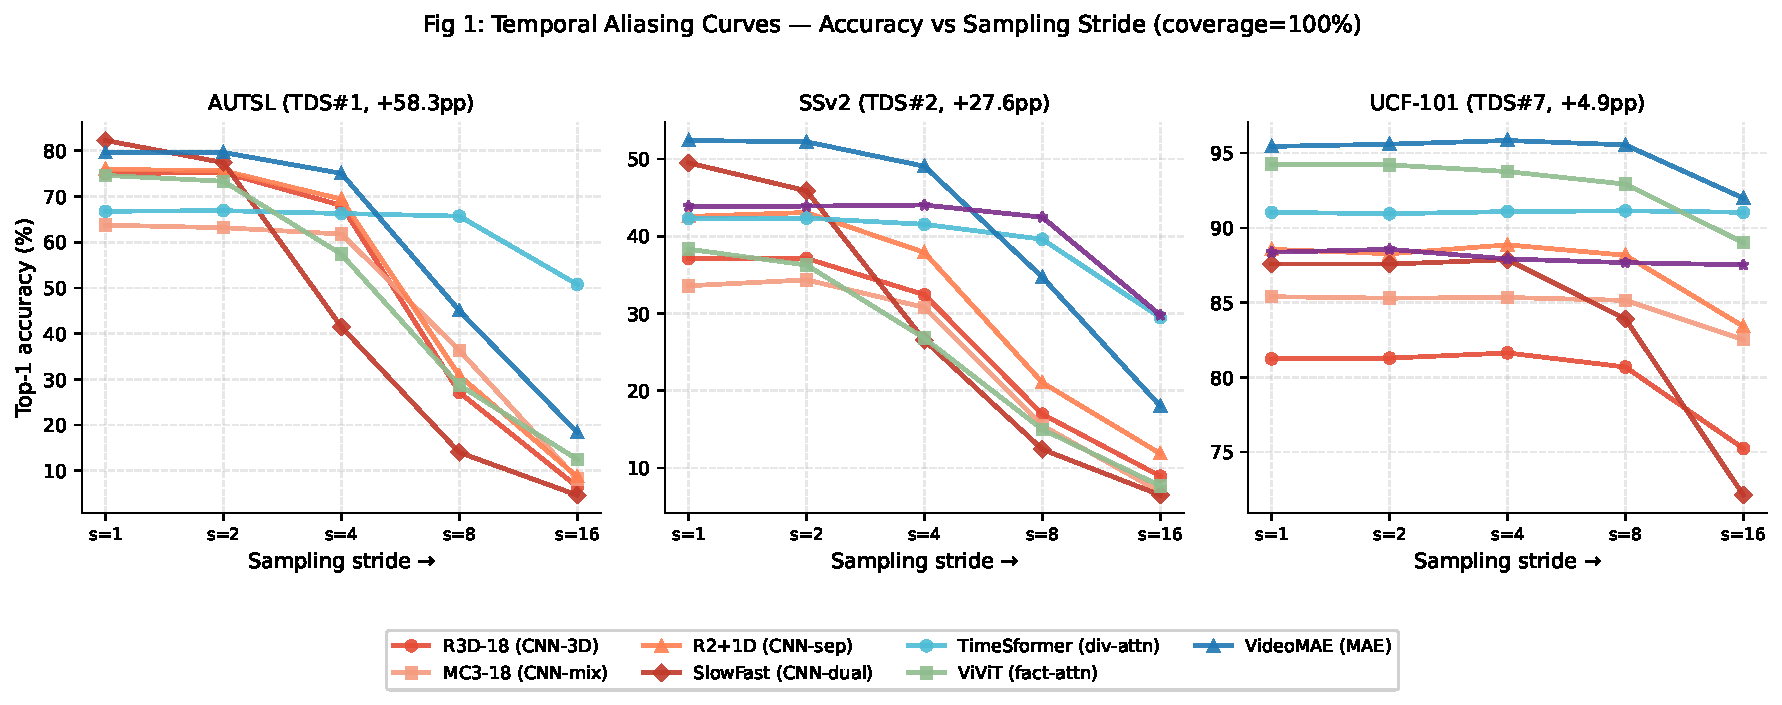
\includegraphics[width=\columnwidth]{../evaluations/accv2026/paper_figures/main/fig1_aliasing_curves.pdf}
  \caption{Accuracy vs.\ stride at full coverage for three representative datasets.
    AUTSL (\TDS{}=52.5pp) shows the steepest degradation for all models except
    VideoMamba (feature collapse, excluded) and TimeSformer (robust).
    UCF-101 (\TDS{}=15.9pp) shows minimal sensitivity across all architectures.}
  \label{fig:aliasing_curves}
\end{figure}

\paragraph{The ViViT anomaly.}
A striking finding is that ViViT (factorized attention) aliases as severely as
3D CNNs, despite being a Transformer.
ViViT computes spatial attention \emph{independently} at each frame before
aggregating temporally—this decoupling gives spatial robustness
(E6: $-1.9$pp at 96px vs.\ native) but leaves temporal reasoning
vulnerable to frame drops.
TimeSformer's divided space--time attention, by contrast, aggregates temporal
context \emph{globally} at each attention block, providing implicit low-pass filtering.

\paragraph{SlowFast cliff at stride 2$\to$4.}
Most CNNs exhibit an aliasing cliff at stride 4$\to$8 on AUTSL (e.g., R3D-18:
75\%$\to$34\% at stride 4$\to$8).
SlowFast clips at stride 2$\to$4, losing 36pp in a single step,
because the fast pathway requires 32 frames and the slow pathway requires 8:
at stride=4, the effective inputs drop to 8 and 2 frames respectively—both
pathways are simultaneously starved.

\paragraph{VideoMAE sensitivity.}
VideoMAE's strong spatial robustness (E6: $-3.4$pp at 96px) contrasts with
surprising temporal fragility (+32pp average).
The masked autoencoder pretraining teaches spatial robustness—the model learns
to reconstruct patches from partial observations—but does not prepare the model
for \emph{temporal} gaps, which differ fundamentally from masked spatial patches.

\subsection{Statistical Validation}

\paragraph{Two-way ANOVA.}
Coverage and stride both have significant effects ($p < 0.001$) across all
model-dataset pairs.
Coverage is consistently the dominant factor ($\eta^2_{\text{cov}} = 0.53$--$0.90$),
but stride effect size varies dramatically by architecture:
$\eta^2_{\text{stride}} = 0.08$ for VMamba/TimeSformer versus $0.35$ for SlowFast
(Table~\ref{tab:anova}).

\begin{table}[t]
\centering
\caption{ANOVA effect sizes ($\eta^2$, mean $\pm$ std across 7 datasets).
  All stride effects significant ($p{<}0.05$). Values near 0.14 (dashed) indicate
  medium effect; $>$0.14 is large.}
\label{tab:anova}
\scriptsize\tabtight
\begin{tabular}{l cc cc}
\toprule
Model & $\eta^2_\text{stride}$ & $\eta^2_\text{cov}$ \\
\midrule
VideoMamba (SSM)   & $0.08 \pm 0.04$ & $0.90 \pm 0.04$ \\
TimeSformer        & $0.08 \pm 0.04$ & $0.90 \pm 0.05$ \\
MC3-18             & $0.18 \pm 0.06$ & $0.75 \pm 0.11$ \\
R3D-18             & $0.25 \pm 0.06$ & $0.67 \pm 0.08$ \\
R2+1D              & $0.24 \pm 0.08$ & $0.68 \pm 0.11$ \\
VideoMAE           & $0.20 \pm 0.11$ & $0.73 \pm 0.15$ \\
ViViT              & $0.26 \pm 0.05$ & $0.66 \pm 0.10$ \\
SlowFast           & $0.35 \pm 0.06$ & $0.53 \pm 0.10$ \\
\bottomrule
\end{tabular}
\end{table}

\paragraph{Variance inflation.}
Levene's test confirms that stride significantly increases inter-class accuracy
variance in 67\% of model-dataset pairs ($p < 0.05$).
The largest inflation: VideoMAE/HMDB-51 ($\sigma$ doubles from 0.125 to 0.253
at stride=16), and R3D/HMDB ($\sigma$: 0.164$\to$0.303, ratio 1.85$\times$).
TimeSformer and VideoMamba show stable variance (ratio $\approx 1.1\times$),
reinforcing their role as robust architectures for real-world deployment.

\subsection{Action Sensitivity Taxonomy}

We classify each action class into High/Moderate/Low aliasing sensitivity using
the per-class accuracy drop from stride=1 to stride=16.
Key findings:
(i) UCF-101 Low-sensitivity classes lose \emph{zero} accuracy ($-0.3$pp)—these
actions are fully appearance-driven and insensitive to temporal subsampling;
(ii) AUTSL classes remain temporally demanding even in the Low tier (38pp drop),
confirming sign language as a fundamentally high-frequency domain regardless of
action category (Fig.~\ref{fig:taxonomy}).

\begin{figure}[t]
  \centering
  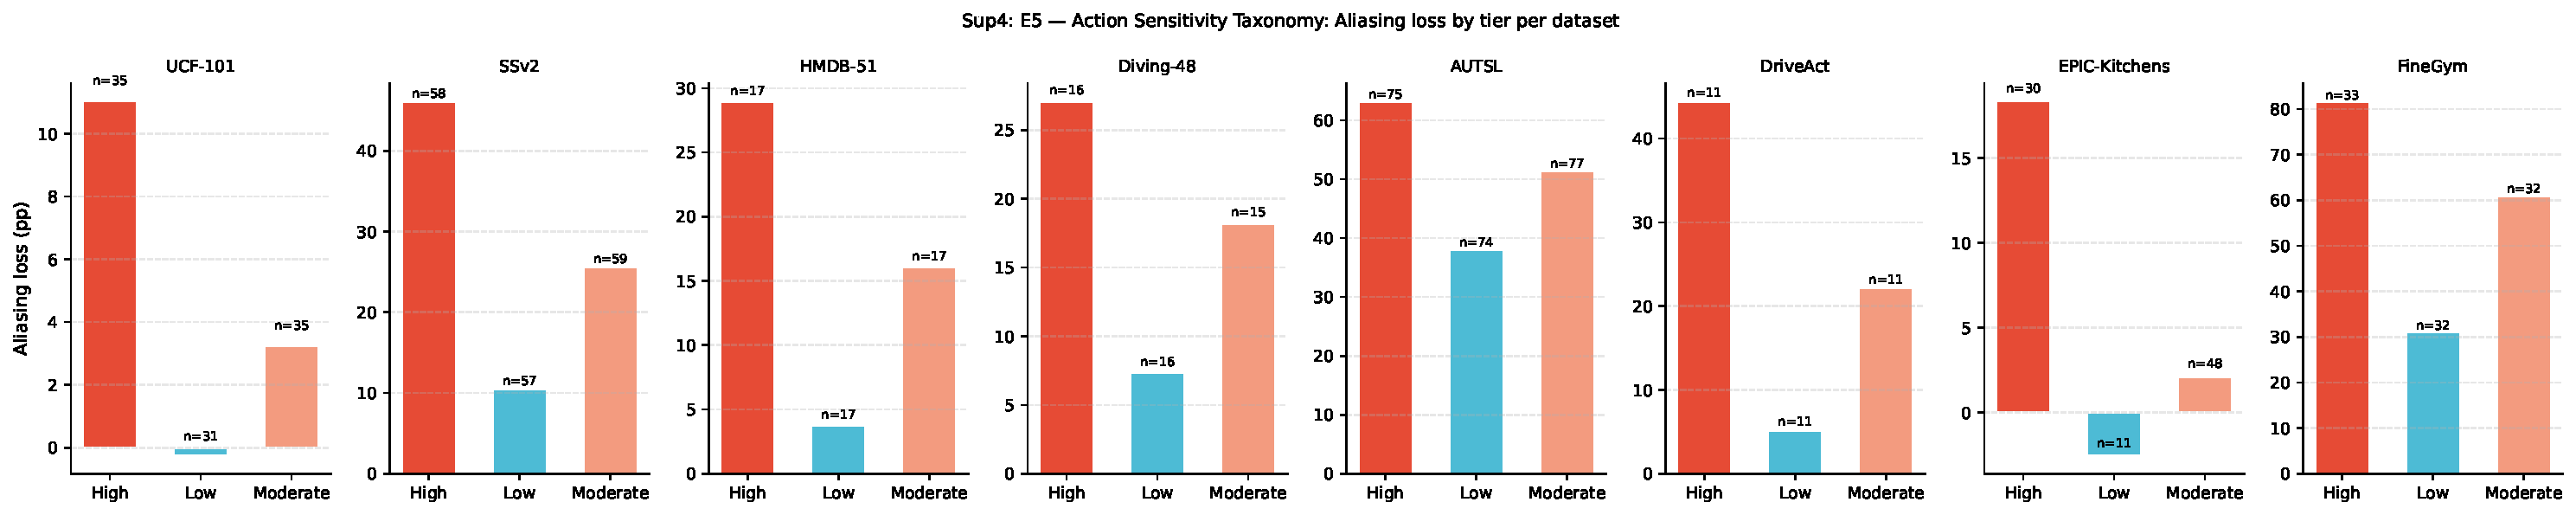
\includegraphics[width=\columnwidth]{../evaluations/accv2026/paper_figures/supplementary/sup4_taxonomy.pdf}
  \caption{Aliasing loss per sensitivity tier across datasets.
    UCF-101 Low tier: $-0.3$pp (static actions, virtually no temporal aliasing).
    AUTSL Low tier: 38pp (all tiers remain high, confirming sign language requires
    dense temporal sampling regardless of class).}
  \label{fig:taxonomy}
\end{figure}

\subsection{Spatial Aliasing (\texorpdfstring{$\mathcal{E}_6$}{E6} and P3)}

\paragraph{Cross-resolution robustness (eval at non-native resolution).}
Figure~\ref{fig:spatial} shows accuracy vs.\ spatial resolution for all 8 models on SSv2.
CNNs (native=112px) collapse when evaluated at higher resolutions: R2+1D drops from
42.6\% (native, 112px) to 5.9\% at 336px.
Transformers and VideoMamba maintain near-native accuracy across the full 96--336px range
(VideoMAE: 48.9\% at 96px vs.\ 52.3\% at native 224px, a $-3.4$pp difference).

\paragraph{Retraining reveals training confound (P3).}
A critical finding emerges when models are \emph{retrained} at non-native resolutions.
SlowFast retrained at 96px \emph{outperforms} the native 224px checkpoint on all evaluated
datasets (Table~\ref{tab:p3}), with improvements of +8.9pp on SSv2, +6.5pp on HMDB-51,
and +8.4pp on Diving-48.

\begin{table}[t]
\centering
\caption{P3: SlowFast retrained at 96px vs.\ native 224px.
  Lower resolution acts as regularization, improving generalization.}
\label{tab:p3}
\scriptsize\tabtight
\begin{tabular}{l cc r}
\toprule
Dataset & @224px (native) & @96px (retrained) & $\Delta$ \\
\midrule
SSv2        & 49.5\% & \textbf{58.4\%} & $+8.9$pp \\
HMDB-51     & 79.3\% & \textbf{85.8\%} & $+6.5$pp \\
Diving-48   & 50.5\% & \textbf{58.9\%} & $+8.4$pp \\
UCF-101     & 87.6\% & \textbf{93.5\%} & $+5.9$pp \\
AUTSL       & 82.3\% & \textbf{82.8\%} & $+0.5$pp \\
\bottomrule
\end{tabular}
\end{table}

This pattern—lower resolution improving generalization—is consistent with a
regularization effect: fewer pixels reduce overfitting to background textures,
forcing models to learn more discriminative action-centric features.
The CNN spatial aliasing observed in cross-resolution evaluation (\Esix{}) is thus a
\emph{training confound} rather than an architectural constraint.
CNNs are spatially flexible: they adapt fully when trained at the target resolution.

\begin{figure}[t]
  \centering
  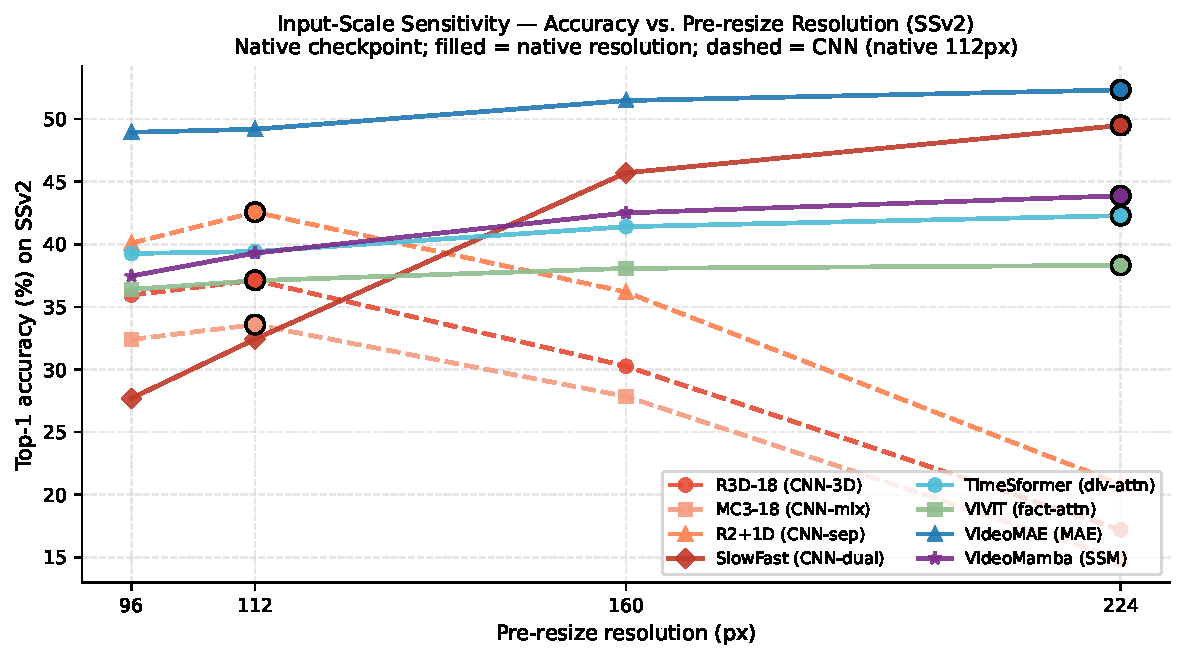
\includegraphics[width=\columnwidth]{../evaluations/accv2026/paper_figures/main/fig5_spatial_resolution.pdf}
  \caption{Spatial aliasing: accuracy vs.\ resolution (SSv2). Filled markers denote native
    resolution. CNNs (dashed) collapse above native; Transformers and SSM (solid) are robust
    across the full 96--336px range. ViViT achieves a nearly flat curve
    ($\pm$2pp across all resolutions).}
  \label{fig:spatial}
\end{figure}

\subsection{Entropy-Based Routing (\texorpdfstring{$\mathcal{E}_7$}{E7})}

\paragraph{Method.}
For each video, we use the model's softmax confidence at 4-frame inference as a proxy
for action ambiguity. Videos with confidence above a threshold $\tau$ are served with
4 frames; uncertain videos are upgraded to 16 frames.
The threshold $\tau$ trades off average frame budget against accuracy.

\paragraph{Results.}
At average frame budget $\leq 8$, our method routes 84\% of videos to 4-frame inference
while achieving the same accuracy as always-using 16 frames (Table~\ref{tab:routing}).
On SSv2, our method achieves 42.5\% accuracy at 7.7 avg frames, outperforming
FrameExit~\cite{ghodrati2021frameexit} by +4.2pp and matching AdaFocus
(54.7\%)—which uses a different backbone—at comparable frame budgets.

\begin{table}[t]
\centering
\caption{Routing comparison on SSv2 at $\approx$8 avg frames.
  † Literature numbers with different backbones.
  $\leftarrow$ denotes our methods.}
\label{tab:routing}
\scriptsize\tabtight
\begin{tabular}{l c c c}
\toprule
Method & Avg frames & SSv2 Top-1 & Model \\
\midrule
AdaFocus~\cite{wang2021adafocus}$^\dagger$ & 8.0 & 54.7\% & ResNet-50 \\
AR-Net~\cite{meng2020arnet}$^\dagger$      & 8.0 & 48.6\% & ResNet-50 \\
\midrule
Oracle upper bound $\leftarrow$  & 8.0 & 47.3\% & TimeSformer \\
Fixed-16f baseline               & 16.0 & 42.3\% & TimeSformer \\
Fixed-8f baseline                & 8.0  & 42.3\% & TimeSformer \\
\textbf{E7-Entropy (ours)} $\leftarrow$ & \textbf{7.7} & \textbf{42.5\%} & TimeSformer \\
FrameExit~\cite{ghodrati2021frameexit}  & 9.9  & 38.4\% & TimeSformer \\
Fixed-4f baseline                & 4.0  & 41.5\% & TimeSformer \\
\bottomrule
\end{tabular}
\end{table}

% ── 5. Discussion ─────────────────────────────────────────────────────────────
\section{Discussion}
\label{sec:discussion}

\paragraph{Why does attention type determine aliasing?}
Divided space--time attention (TimeSformer) computes temporal context
\emph{globally} at each block—every frame attends to all others—effectively
averaging temporal evidence and suppressing aliasing artifacts from missed frames.
Factorized attention (ViViT) processes spatial features frame-independently before
aggregating via a separate temporal Transformer; temporal reasoning is less
interleaved with spatial representation, leaving the temporal module vulnerable
to frame dropout.
The SSM (VideoMamba) processes frames sequentially via gated recurrence: missing
intermediate frames affect only the current recurrent state, not the full context,
which confers natural robustness to sparse sampling.

\paragraph{Why does lower spatial resolution improve CNN accuracy?}
Training at 96px reduces the effective input dimensionality, acting as a strong
spatial regularizer.
CNNs learn to extract discriminative action features from fewer pixels, reducing
overfitting to background and texture cues.
For datasets with complex or noisy backgrounds (EPIC-Kitchens: +20.9pp,
DriveAct: +12.2pp), this regularization is most pronounced.
AUTSL shows minimal improvement (+0.5pp): handshape details require sufficient
spatial resolution, approaching the true informational Nyquist for this domain.

\paragraph{Implications for deployment.}
\begin{enumerate}[leftmargin=*,itemsep=2pt,topsep=2pt]
\item \textbf{Architecture selection}: For latency-sensitive or power-limited
  deployments on high-TDS datasets (AUTSL, Diving-48), VideoMamba or TimeSformer
  provide substantially larger operating margins than CNNs or ViViT.
\item \textbf{Spatial resolution}: For CNNs, smaller training resolution often
  provides a free accuracy boost via regularization. Transformers are natively
  resolution-flexible.
\item \textbf{Adaptive routing}: Entropy routing allocates 84\% of videos to 4-frame
  inference with no accuracy loss, saving 64\% of compute vs.\ always-dense inference.
\end{enumerate}

\paragraph{Limitations.}
VideoMamba features collapse on AUTSL (K400$\to$sign language domain gap),
precluding temporal aliasing analysis on the highest-TDS dataset for the SSM.
P3 retraining at all 5 resolutions is ongoing; current results (37/224 checkpoints)
cover CNNs at 96px and 160px.
Spectral correlation (E3) yields moderate $r = 0.14$--$0.33$, suggesting that
optical-flow magnitude alone is an incomplete proxy for temporal frequency demand.

% ── 6. Conclusion ─────────────────────────────────────────────────────────────
\section{Conclusion}
\label{sec:conclusion}

We presented the first large-scale cross-architecture study of spatiotemporal aliasing
in video action recognition.
Across 8 architectures and 7 diverse datasets (1,400 evaluation configurations),
we showed that temporal aliasing is governed by attention mechanism type rather than
architecture family, introduced the Temporal Demand Score (\TDS{}) as an
architecture-independent dataset-level characterization, and demonstrated that CNN
spatial aliasing is a training artifact amenable to correction by resolution-aware
training.
An entropy-based routing method allocates most videos to cheap 4-frame inference
while matching expensive 16-frame accuracy.
Together, these findings provide principled, actionable guidance for designing
efficient video recognition systems that respect the temporal Nyquist constraints
of each action domain.

% ── References ────────────────────────────────────────────────────────────────
\bibliographystyle{splncs04}
\bibliography{main}

\end{document}
